\chapter[Bartok and \textit{Romanian Folk Dances}, Sz. 56, BB 68]{Béla Bartók - \textit{Romanian Folk Dances}, Sz. 56, BB 68 (1915)}

Bela Bartok (1881-1945) was a Hungarian ethnomusicologist\footnote{This involves the study of music of world culture, both of the past and present, with an emphasis on the cultural, racial, and other influences, and affects on the music.}, pianist, and composer. Bartok was born in the Austro-Hungarian Empire, in a small Hungarian city in what is present-day Romania. With parents who were teachers and amateur musicians, Bartok went on to study music at the Hungarian Royal Conservatory of Music \autocite{Burkholder_Grout_Palisca_2014}. He returned to the Conservatory in 1907 to teach, but withdrew from public musical life in 1912\autocite{Gillies}. As a teacher, Bartok did not create a distinctive ``school'' for his students, as other teachers had, disinterested in teaching piano technique or other methods. In that time, Bartok only contributed and co-authored almost 50 piano pieces (Zongoriaskola, ``Piano Method'') in 1913, for piano technique at the school\autocite{Gillies}. These pieces began his ethnomusicological studies which would become his primary method of professional musical progress and income over the next several years. Later, Bartok began searching for innately Hungarian music, leading him to collect and study peasant music from many places. Bartok would go on to publish many songs and dances, with roots in Hungary, Romania, Slovakia, Croatia, Serbia, and Bulgaria, from his travels through central Europe, Turkey, and North Africa \autocite{Burkholder_Grout_Palisca_2014}. Within the new field of ethnomusicology, Bartok edited various collections and wrote books and articles which would establish him as a leading scholar in the field. To him, Hungarian peasant music represented the music of the country better than other types of music to come out of Hungary. This view was radical for a short time, as Hungary was ruled by an urban, German-speaking elite class, but eventually prevailed \autocite{Burkholder_Grout_Palisca_2014}. Based on peasant songs and dances, he created pieces, imitating the melodies, rhythms, and other characteristics found, blending them with more classical elements from his time at studying classical music. 

Around 1908, Bartok achieved a distinctive personal style, as his compositions introduced a new aspect to the piano. It was treated as a percussive instrument rather than a melodic one \autocite{Burkholder_Grout_Palisca_2014}. When World War I (WWI) began in 1914, Bartok's travels to collect folk music became near impossible \autocite{Gillies}. Instead, Bartok turned to arranging and creating folk-based music. In 1915, the Román nepi táncok (``Romanian Folk Dances'', BB 68) was composed, and in 1918, two Hungarian piano sets--Tizenöt magyar parasztdal (``15 Hungarian Peasant Songs'', BB 79), and ``Three Hungarian Folk Tunes'', BB80b--were finished \autocite{Gillies}. In the decade after WWI, Bartok pushed towards the previously-defined limits of musical dissonance and tonal ambiguity. In his synthesis of peasant folk music with classical music, there became an emphasis on the characteristics the two styles shared, and the distinctions each had. In both peasant folk songs and classical music, pieces will typically have a tonal pitch center, and will use diatonic and other scales, with melodies built from repeated motives \autocite{Burkholder_Grout_Palisca_2014}. From the classical side, Bartok pulled on contrapuntal and formal structures and procedures, with the fugue and sonata as examples. Then, from the folk songs, he pulled the irregular meters and complex rhythms, mixed modes and modal scales, and the defining melodic structure and specific ornamentation to folk songs \autocite{Burkholder_Grout_Palisca_2014}. Music by Bartok thus became simultaneously complex in counterpoint--more than Bach's-- and rhythmically complex with more ornamentation than the folk songs he referenced. The dissonance and harmonic strategies used were also based on the mixed concepts from the two musical styles. For example, Bartok frequently uses second and fourth chords\footnote{In a triadic chord, these chords would include the tonic, second, and fifth, and then the tonic, fourth, and fifth notes of the chord, respectively.}. Aesthetically, from a classical music perspective, Bartok placed himself somewhere in between Beethoven (in terms of artistic and harmony style), and Bach (in counterpoint). Later, in 1926, the styles of Schoenberg--expressionism\footnote{A trend which is common in the twentieth-century, in which composers attempt to convey emotional value and meaning through music, above all else. Musically, expressionism will often include a higher level of dissonance than non-expressionist music, extreme dynamic contrast, angular melodies with large leaps, more to bring the intended emotion across to the listener.}-and Stravinsky--neoclassicism\footnote{A trend also commonly found in the twentieth-century, in which composers sought to return to the ``golden age'' or so of Classical-era music. This return would be to the aesthetic characteristic associated with the Classical era, including balance, clarity, and emotional restraint.}--were also emulated \autocite{Gillies}.

\section{Romanian Folk Dances, Sz. 56, BB 68}

This mixture between elements of peasant folk dances from Romania, Hungary, Bulgaria, and other countries, and traditional classical music is clear in Bartok's ``Romanian Folk Dances''. The original name for ``Romanian Folk Dances'' included the phrase ``From Hungary'' at the end, as the pieces are based on folk songs Bartok heard during his time traveling to Transylvania \autocite{Burkholder_Grout_Palisca_2014}. The title was later changed when Transylvania became part of Romania in 1920, dropping the ending ``From Hungary''. Each piece here will be referred to its most well-known title (in Romanian), with the English translation in parentheses.

\subsection{Jocul cu bâtă (``Stick Dance'')}

\begin{figure}
  \centering
  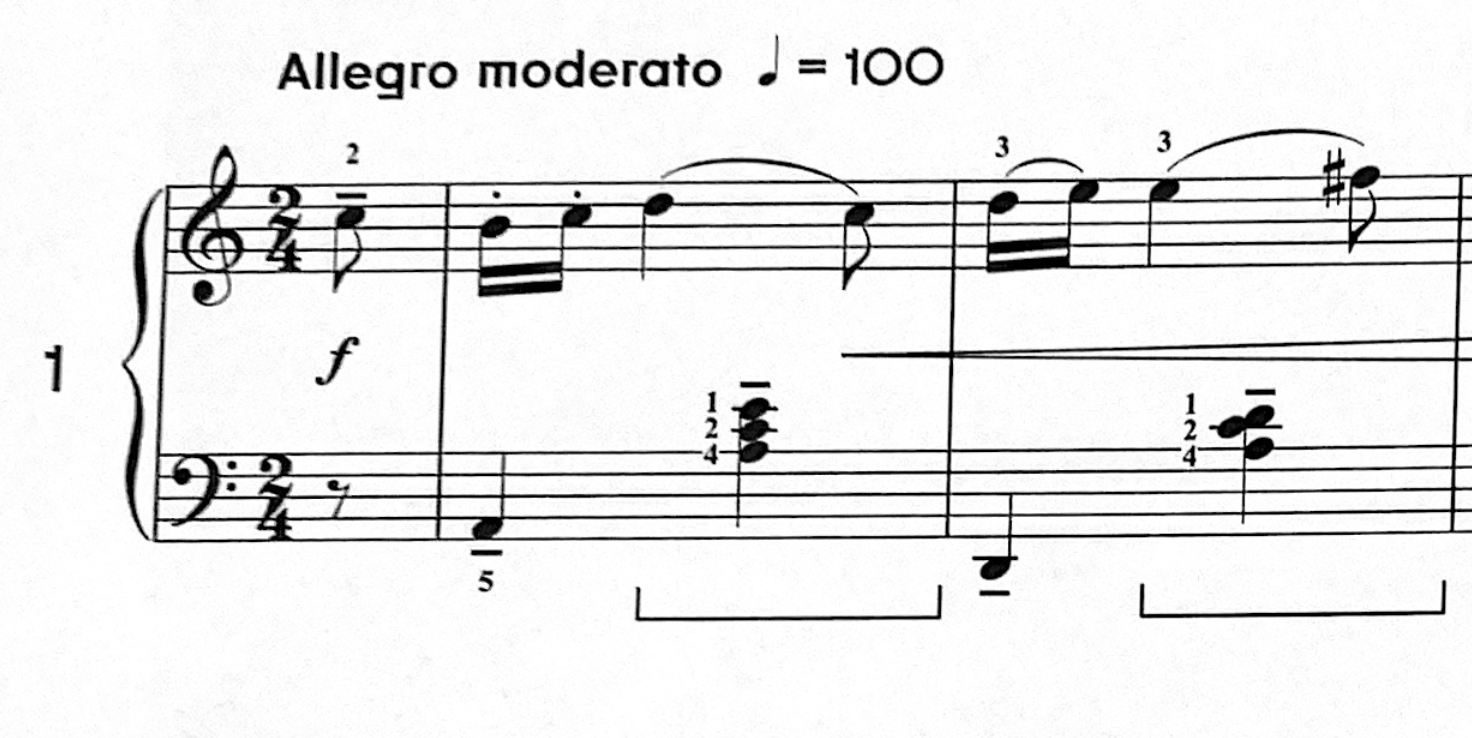
\includegraphics[width=0.5\textwidth]{bartok-stick-dance-first-two-bars.jpg}
  \caption[The first two bars, in ``Jocul cu bâtă'' of  Bartok's \textit{Romanian Folk Dances} Sz. 56, BB 68]{The first two bars of ``Jocul cu bâtă''}
  \label{fig:bartok-stick-dance-first-two-bars}
\end{figure}

\begin{figure}
  \centering
  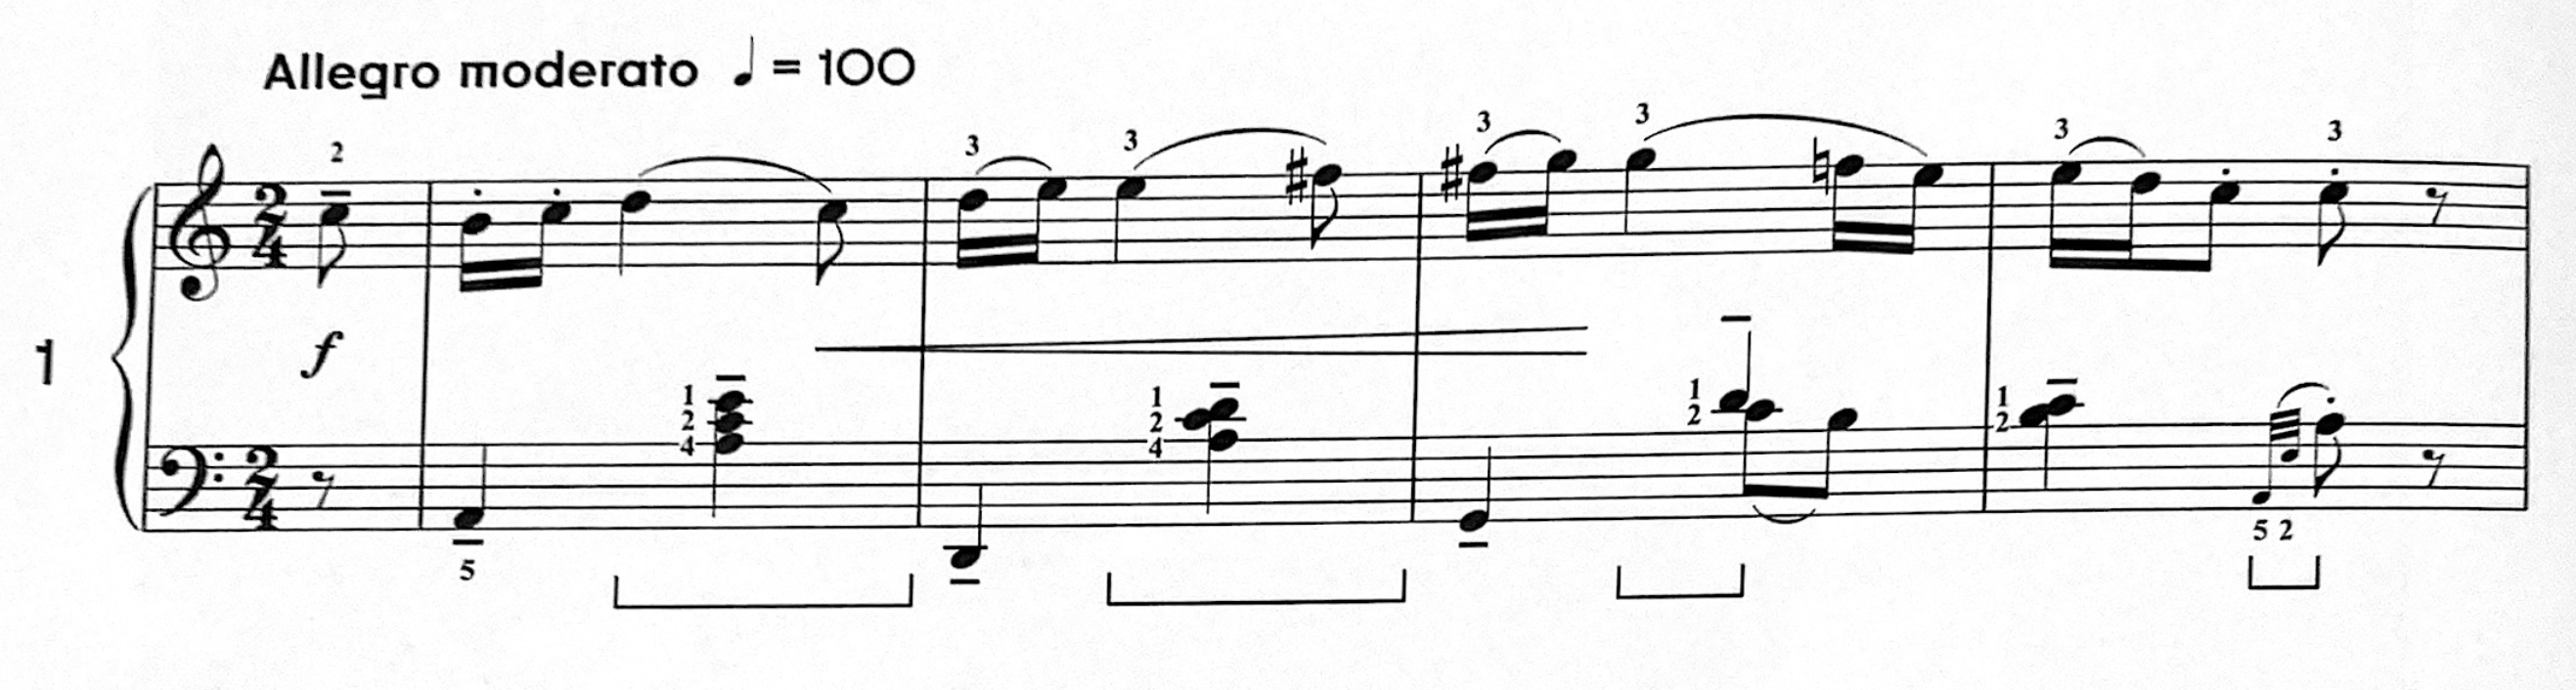
\includegraphics[width=\textwidth]{bartok-stick-dance-first-line.jpg}
  \caption[The first line of ``Jocul cu bâtă'' of Bartok's \textit{Romanian Folk Dances} Sz. 56, BB 68]{The first line of ``Jocul cu bâtă''}
  \label{fig:bartok-stick-dance-first-line}
\end{figure}


This piece, titled ``Jocul cu bâtă'' or ``Stick Dance'' in English, is a stick dance meant to be energetic and upbeat. As the longest piece of the six in this set, this dance was performed by menu solo, as a solo dance which consists of kicking the ceiling of the room in which the dance takes place \autocite{Weissmann_1969}. These details of the dance are clearly seen in the melody. In of itself, the melody, as in  in Figure \ref{fig:bartok-stick-dance-first-two-bars}\autocite{Lung_2016}, is not as danceable as the title suggests. Instead, the melody is more elegant in sound, with the rhythm not lending itself easily to a dance-like sound. In the first line of the dance in Figure \ref{fig:bartok-stick-dance-first-line}\autocite{Lung_2016} the rhythm of the right hand stutters in a syncopated melody. These articulations to the melody convey to the listener that this piece is a specific type of dance not commonly found, and to the performer the specific stylistic traits found within a stick dance. In the score, as in \ref{fig:bartok-stick-dance-first-line}\autocite{Lung_2016}, Bartok marks the articulations clearly. Within the first line itself, there are dynamic markings (the \textit{forte} and crescendo denoting that the volume of the beginning starts loud, and gets louder), and phrasing markings, detailing which notes should be connected to each other. Later in the piece, there are also other markings for the stick dance's intended style: accent marks, the usage of \textit{sforzando}, \textit{tenuto} and more. Bartok carefully guided the performer to the specific idea which he wanted the music to contain, doing so by also including the specific metronome tempo marking for the quarter note (80 beats per minute would be the equivalent to one quarter note, as seen in Figure \ref{fig:bartok-stick-dance-first-two-bars}\autocite{Lung_2016}).

\begin{figure}
  \centering
  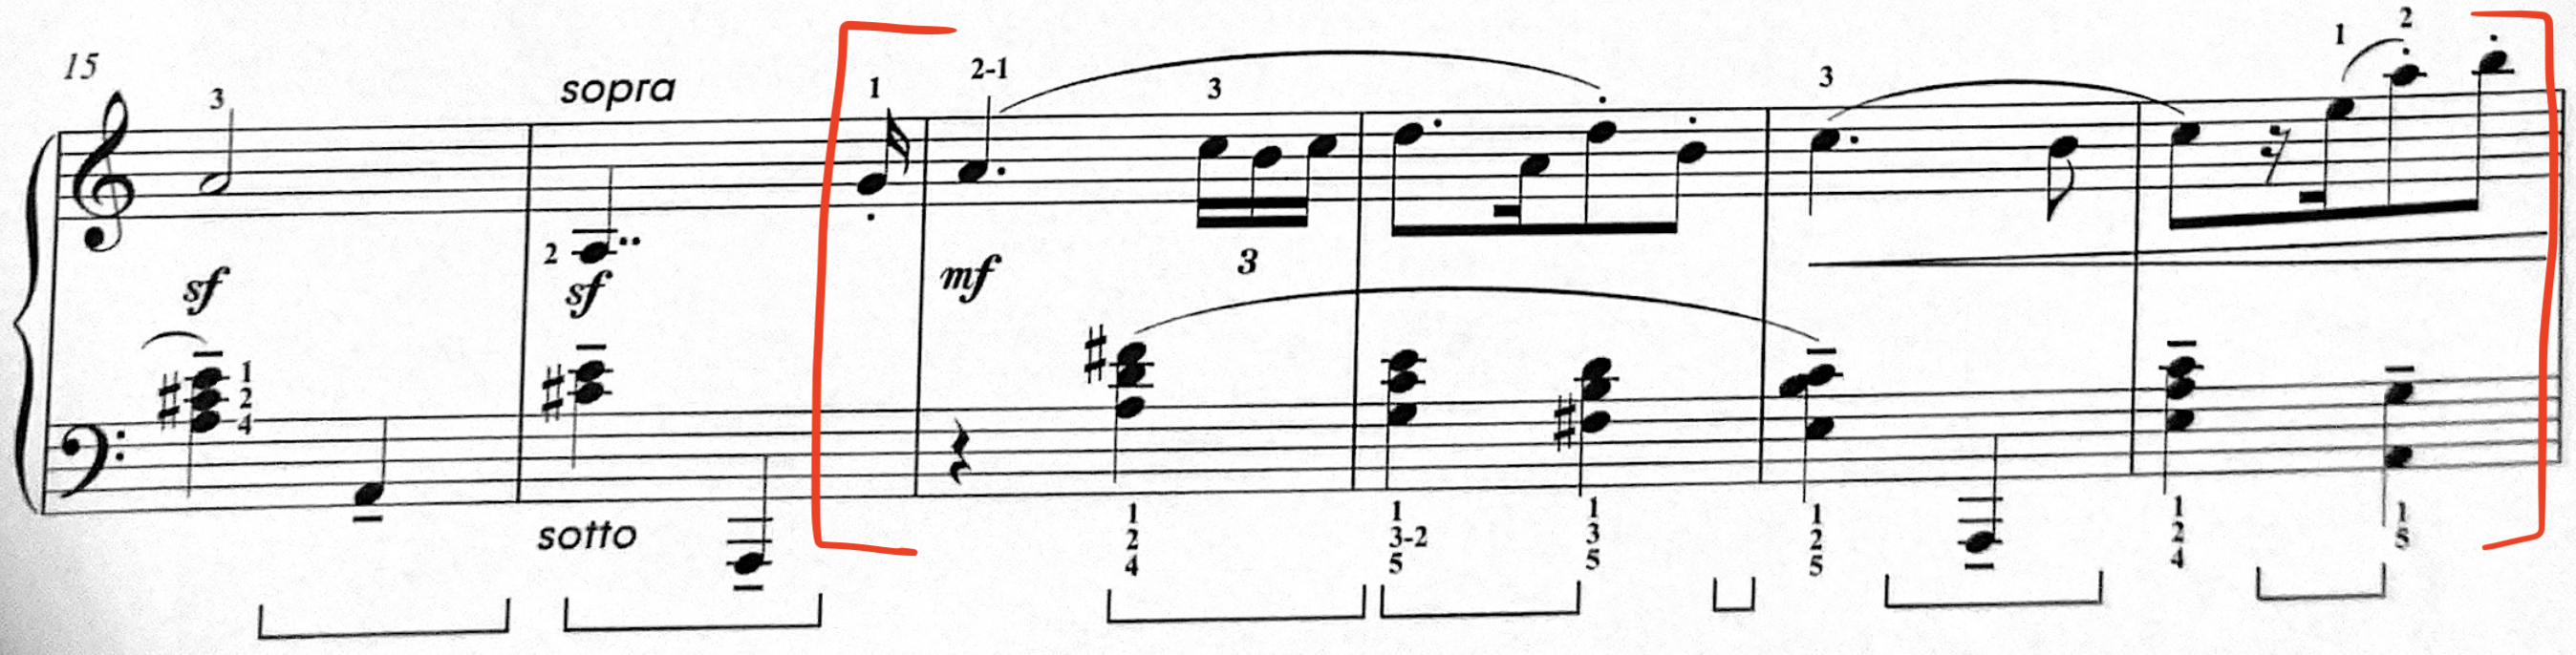
\includegraphics[width=\textwidth]{bartok-stick-dance-b-section.jpg}
  \caption[The B Section, of ``Jocul cu bâtă'' in Bartok's \textit{Romanian Folk Dances, Sz. 56, BB 68}]{The B section of ``Jocul cu bâtă''}
  \label{fig:bartok-b-section}
\end{figure}


Structurally, the piece is in binary form. In the A section, which lasts from bars 1-15, the first four bars (Figure \ref{fig:bartok-stick-dance-first-line}\autocite{Lung_2016}) feature a clear suggestion Bartok wanted. In this first phrase, the first full bar features two sixteenth notes played staccato, followed by a quarter note slurred into an eighth note. This phrase has the dynamic \textit{forte}, signaling to the dancer of the piece that the music is starting, and uses the staccato of the first two notes to signify that this piece will be energetic. As opposed to the rhythms found in the B section, this section is gentler, and more dance-like, but only in comparison to the B section. 

The second measure of the fourth system (the fourth line of the piece) begins the piece's B section. As in Figure \ref{fig:bartok-b-section}\autocite{Lung_2016}, the rhythm changes to include dotted rhythms, marked here in red brackets. The first full measure of this bracketed section features one set of sixteenth note triplets. These notes are meant, as Bartok notates, to sound as ornamentation and support for the dancers, instead of a rhythmic tool solely for the instrumentalist. The set of triplets is slurred with the dotted quarter note before it, and the dotted eighth and sixteenth notes after it. As the triplets are centered around a primary pitch of C, it would be difficult for the instrumental accompanist for this piece to play it directly as written. The dotted rhythms of the eighth and sixteen notes which appear later in the B section may imitate the sounds of the dancers hitting the ceiling with the stick.

\subsection{Brâul (``Sash Dance'')}

\begin{figure}
  \centering
  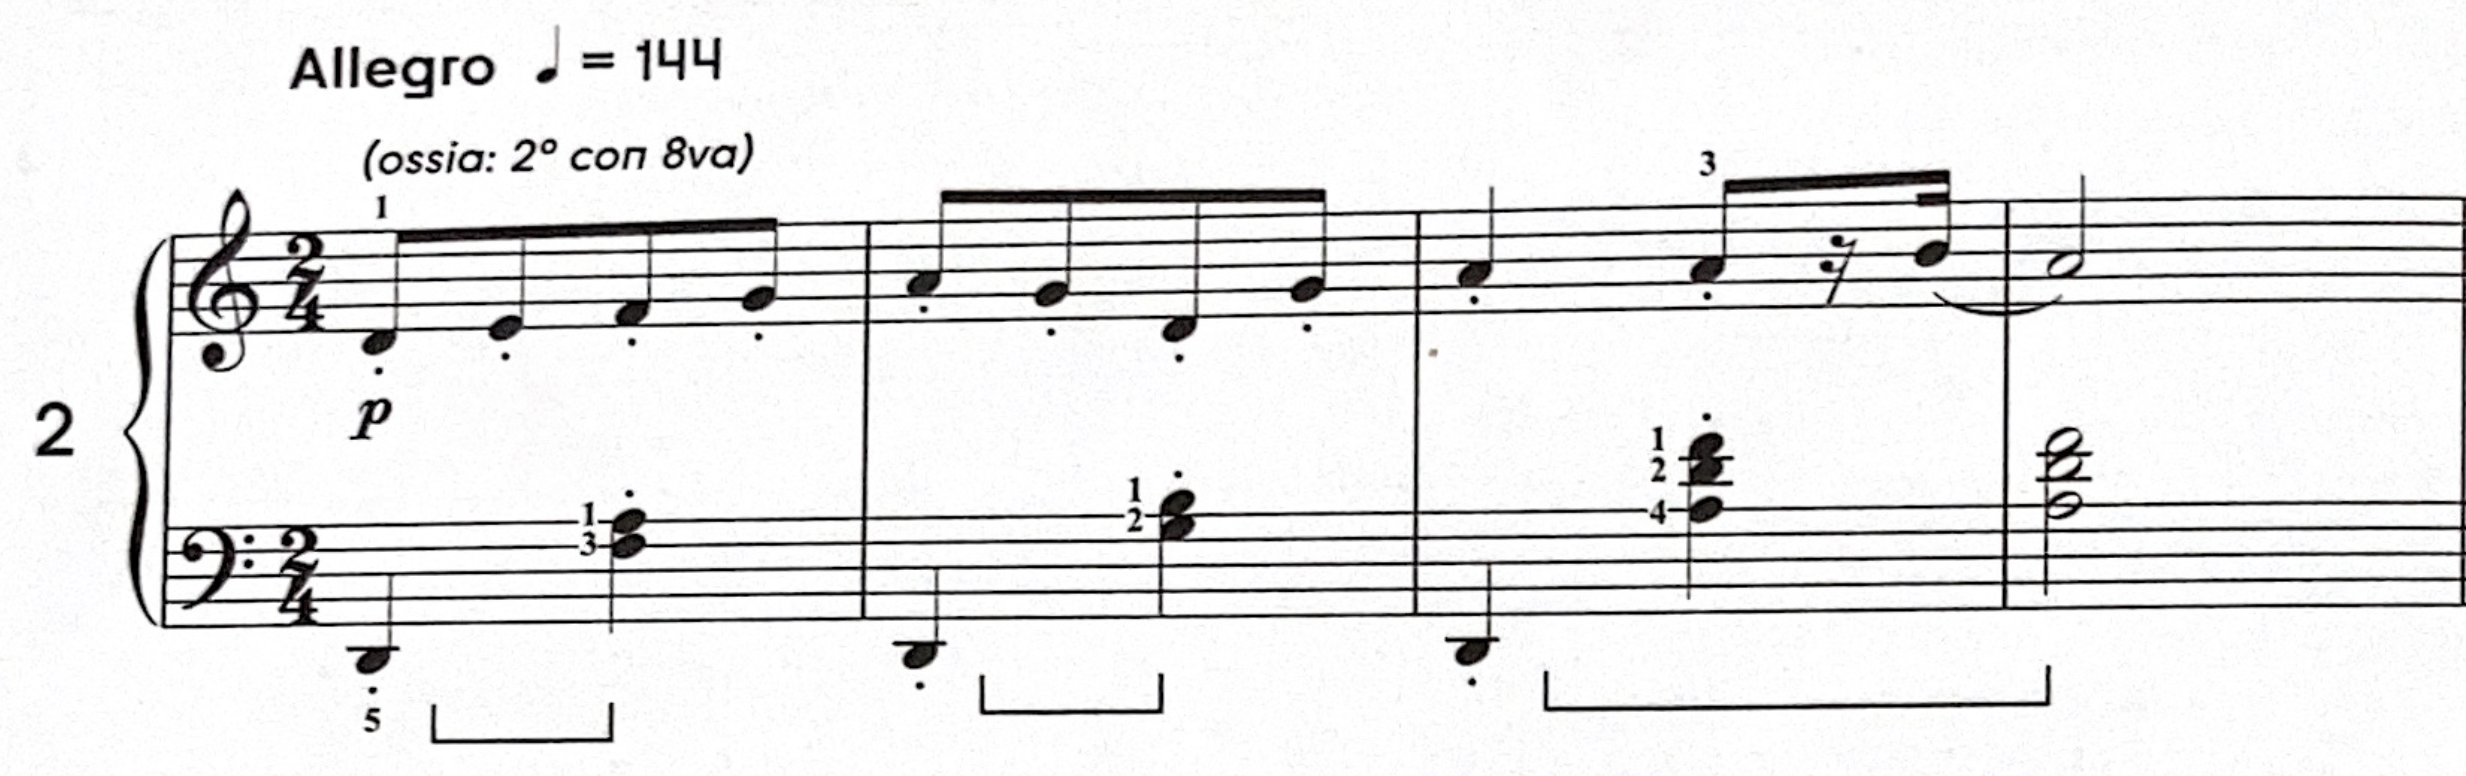
\includegraphics[width=\textwidth]{bartok-waistband-dance-tempo-marking-and-dynamic.jpg}
  \caption[An example of the open interpretation in ``Brâul'' of Bartok's \textit{Six Romanian Folk Dances}, Sz. 56, BB 68]{Examples of Open Interpretation in ``Brâul''}
  \label{fig:bartok-waistband-dance-interpretation}
\end{figure}

The second of the dances in the set, Brâul (``Sash Dance''), is the shortest dance, at only two systems long. A Brâul is a typical dance out of Romania, in which traditionally a sash or other type of waistband is used as an accessory in the dance. It is a fast and energetic dance, with an undertone of sadness to the tune. This undertone is reflected in the freedom Bartok has given the performer, as in Figure \ref{fig:bartok-waistband-dance-interpretation}\autocite{Lung_2016}. The only non-rhythmic aids Bartok gives the performer is a metronome tempo marking for the quarter note, and a note to repeat the whole piece again at the end, introducing a slow \textit{ritardando} at the end. Though there is no key signature, we see that through the first bar of the piece, the left-hand signals that the tonic key of the piece will be D Minor. At the beginning of the piece, it is already energetic, with the Allegro tempo marking, and the quarter note equal to 144 beats per minute (Figure \ref{fig:bartok-waistband-dance-interpretation}\autocite{Lung_2016}). In its rhythm, each note is mostly to be played \textit{staccato}, with only a few notes played slurred, or held out with a note longer than the length of a quarter note. The melody matches this bouncy feel which the rhythm gives the piece. After each phrase, the motion of the piece as a whole stops for a moment. As in Figure \ref{fig:bartok-waistband-dance-interpretation}\autocite{Lung_2016}, there is clear, continuous motion as the melody continues on. But, as the left hand's rhythm becomes smoother to signal a shift to a longer note, so does the melody, containing a thirty-second note before coming to a temporary close on a half-note. 

\subsection{Pe loc (``In One Spot'')}

\begin{figure}
  \centering
  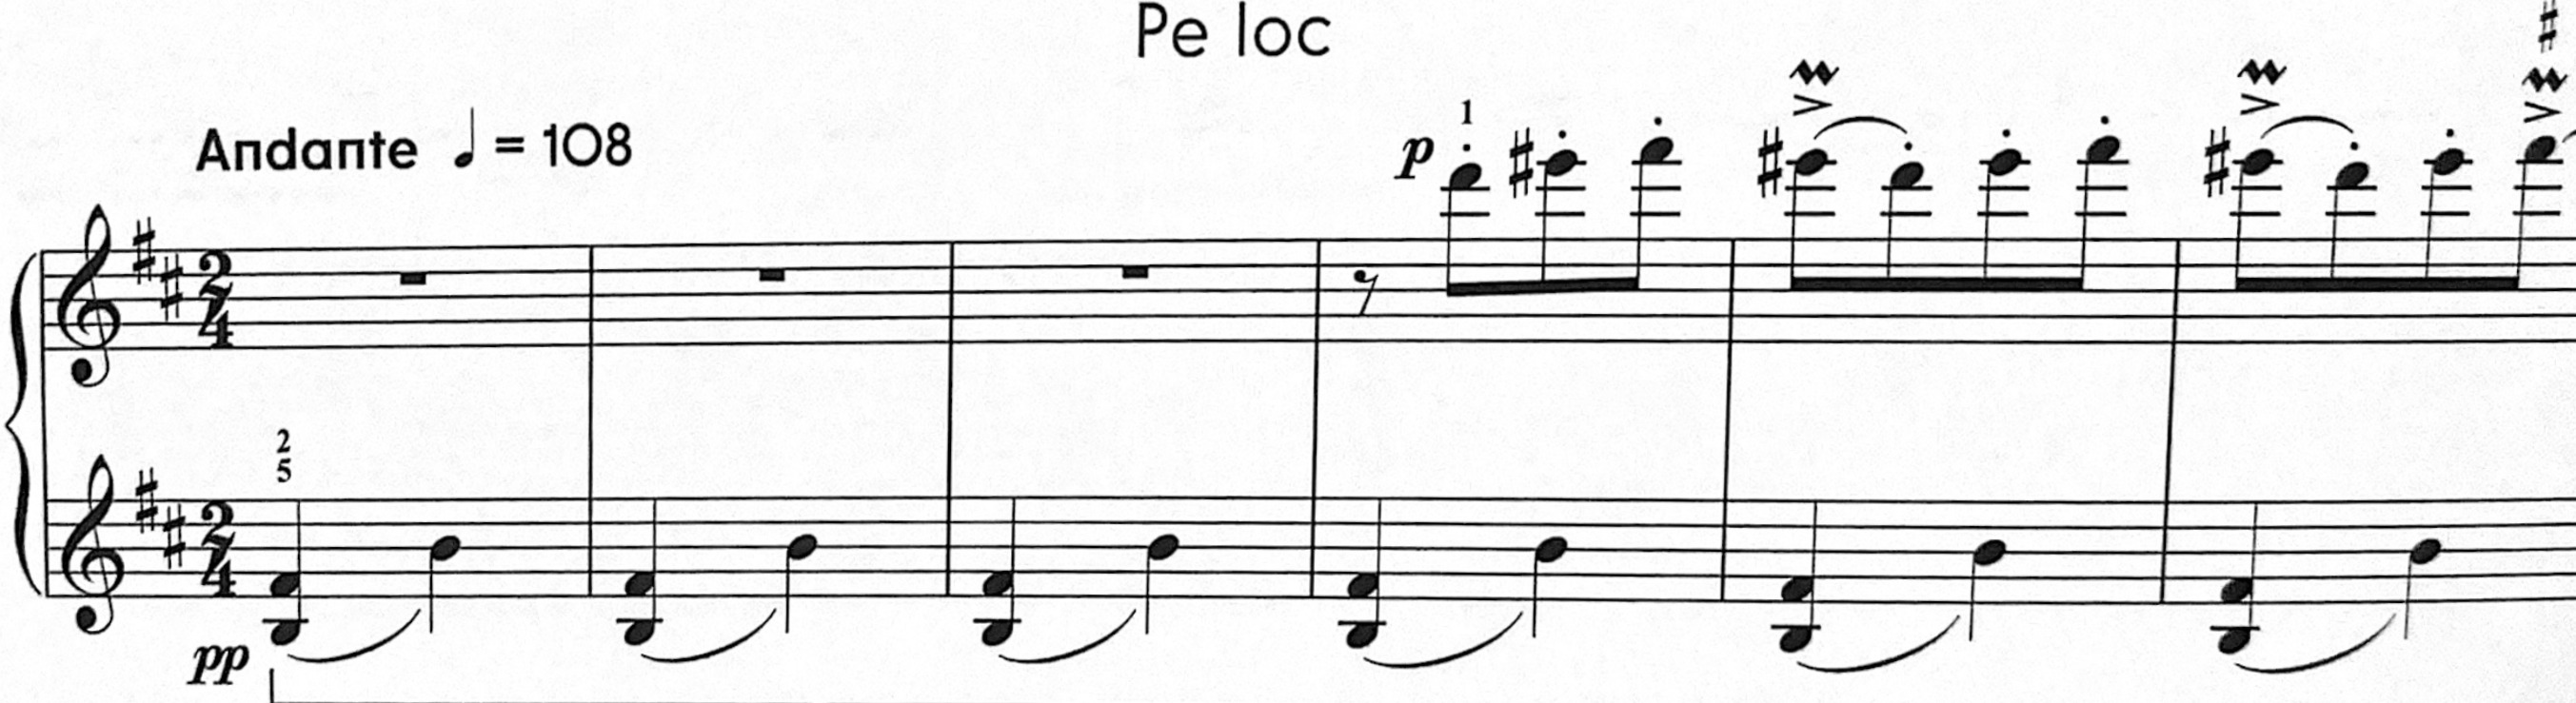
\includegraphics[width=\textwidth]{bartok-one-spot-beginning.jpg}
  \caption[The beginning of ``Pe loc'', in Bartok's \textit{Six Romanian Folk Dances}, Sz. 56, BB 68]{The beginning of ``Pe loc''}  
  \label{fig:bartok-one-spot-beginning}
\end{figure}

The music of the second dance, ``Brâul'', flows directly into the third dance, ``Pe loc'' (``In One Spot''). It is much slower than ``Brâul'', giving a greater contrast. The beginning of the piece, as in Figure \ref{fig:bartok-one-spot-beginning}\autocite{Lung_2016}, features an overall slower melody and accompaniment. The range that the right-hand's melody plays is confined to small intervals, narrow enough to fit within the one high octave in which it is played. It is also meant to be played slowly, marked with the \textit{Andante} tempo marking, and the metronome marker of 90 beats per minute for the quarter note. The accompaniment that is found in the left hand is that of a droning sound, as the only movement within the piece is in the melody. This gives the dance the idea that it is to be performed in one spot, as both the right hand's melody and left hand accompaniment stay within the range of an octave.

\begin{figure}
  \centering
  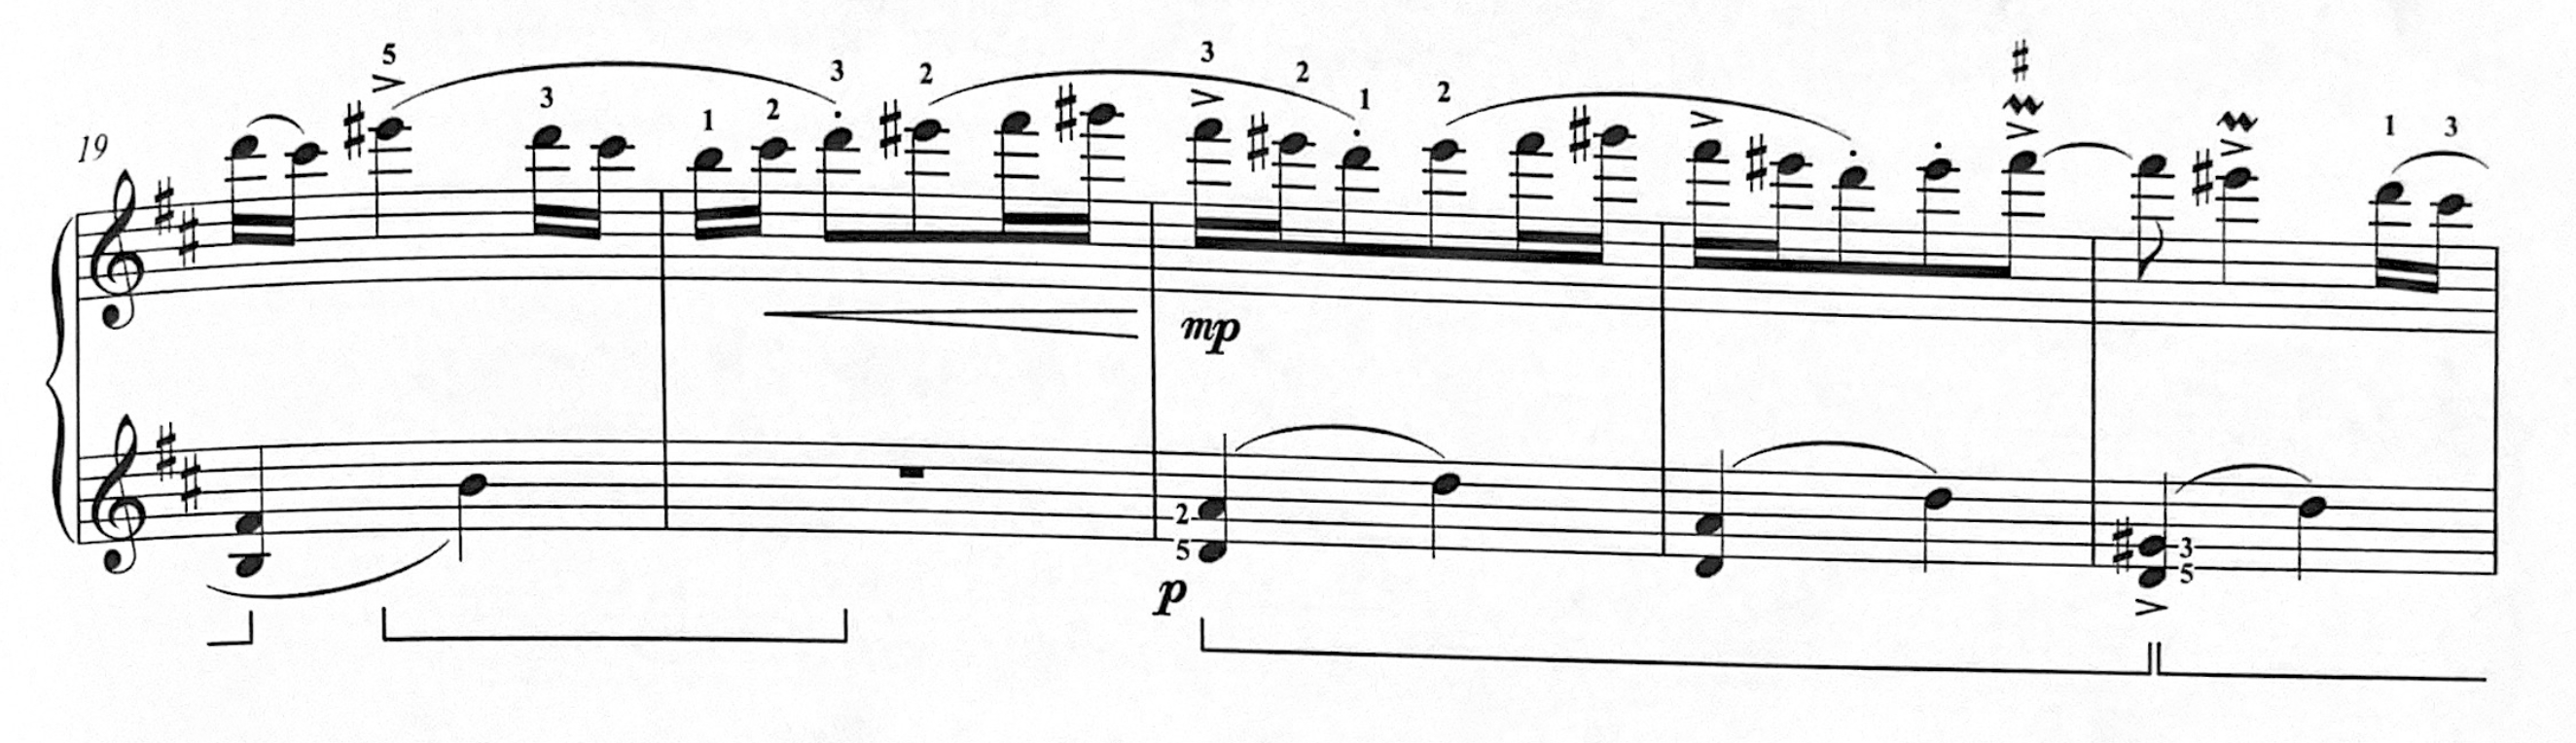
\includegraphics[width=\textwidth]{bartok-one-spot-b-section.jpg}
  \caption[The B section of ``Pe loc'', of Bartok's \textit{Romanian Folk Dances, Sz. 56, BB 68}]{The B section in ``Pe loc''}
  \label{fig:bartok-one-spot-b-section}
\end{figure}

The dance is in binary form, with sections A (measures 1-18) and B (measures 19-40). The A section starts the dance in the key of B Minor, but also features the use of the raised fourth scale degree, with the E\musSharp{} instead of E, as seen in Figure \ref{fig:bartok-one-spot-beginning}\autocite{Lung_2016}, marked in red. When E\musSharp{} is played before or after the note D, the augmented second interval is created. This augmented second interval--in which the typical one whole tone distance between one note and the next is increased by a semitone, and the resulting interval containing the distance of one and a half tones--is what creates the gypsy-like, rooted sound quality, containing the interval typical of many Middle Eastern instrumental pieces, the augmented second. The B section shifts the tonal center of the dance, modulating to D Major, the relative major key to B Minor, the tonic key found in the A section. This is found in Figure \ref{fig:bartok-one-spot-b-section}\autocite{Lung_2016}, where the left-hand accompaniment shifts to center around the chord of D Major. Similar motivic material, for both melody and harmony, is used as it was found in the A section.

\subsection{Buciumeana (``Dance from Bucsum'')}

\begin{figure}
  \centering
  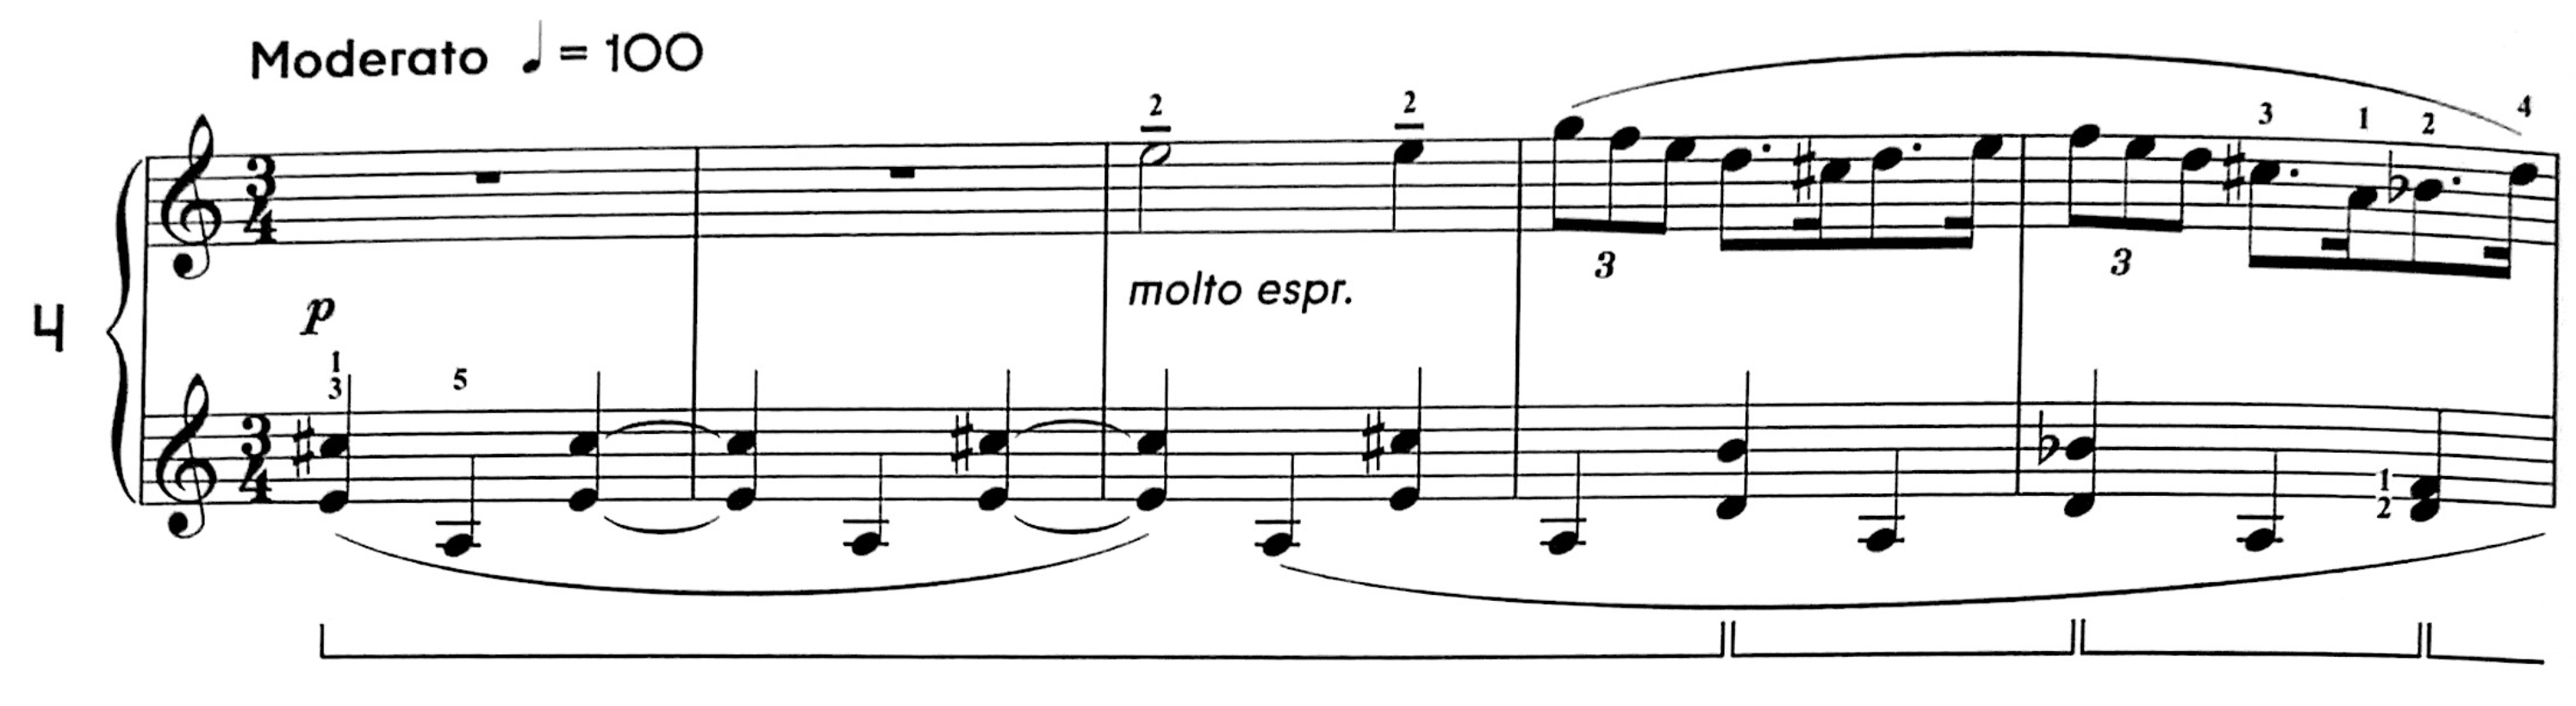
\includegraphics[width=\textwidth]{bartok-dance-four-first-line.jpg}
  \caption[The first line of ``Buciumeana'' of Bartok's \textit{Romanian Folk Dances}, Sz. 56, BB 68]{The first line of ``Buciumeana''}
  \label{fig:bartok-dance-four-first-line}
\end{figure}


The fourth dance in this set, ``Buciumeana'', comes from modern day Bucium, in Alba county in Romania. It is meant to be played slow, as evident by Figure \ref{fig:bartok-dance-four-first-line}\autocite{Lung_2016}, in which the given tempo marking is \textit{Moderato}, with quarter notes to be played at 100 beats per minute. Because it is slow, it has a childlike simplicity to it. Both rhythm and melody are simple in sound, with the left-hand accompaniment treating solely quarter notes and quarter rests. An important feature of this dance to notice, as in Figure \ref{fig:bartok-dance-four-first-line}\autocite{Lung_2016}, is that in the right hand's melody, the shape of the melody is downwards. Every phrase in the melody goes in a downwards direction, giving the dance an almost wistful and youthful sound. This dance is constructed in binary form, with section A from measures 1-10, and section B from measures 11-18. Both sections are in the piece's tonic key of A Major, but treat slightly different thematic material. 

\begin{figure}
  \centering
  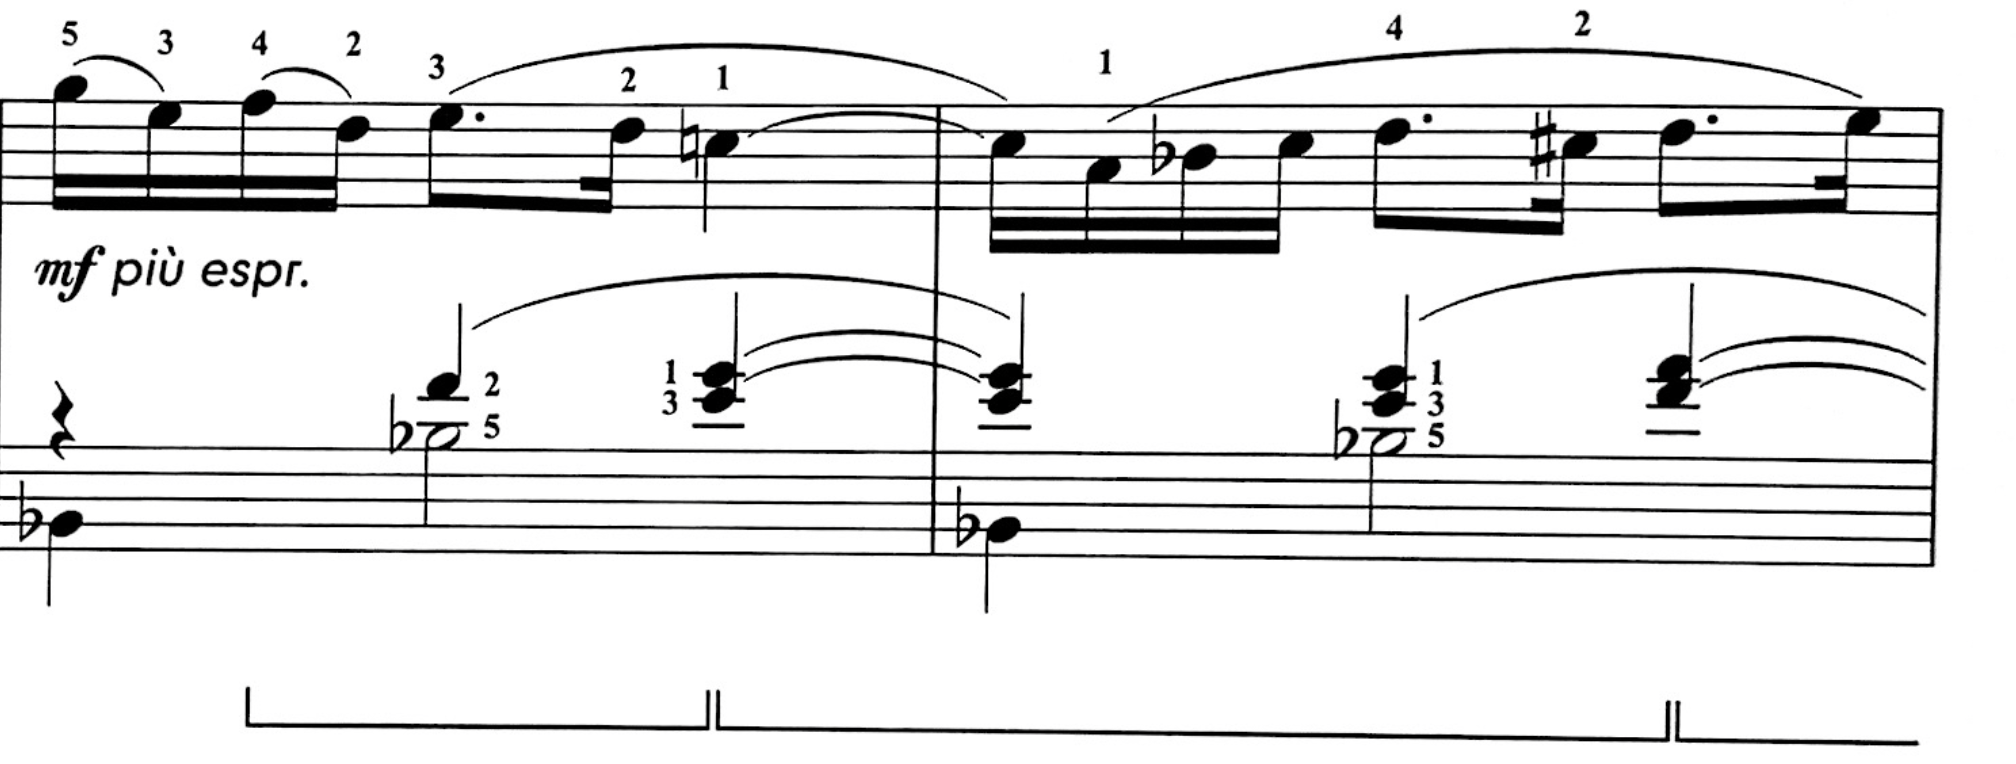
\includegraphics[width=\textwidth]{bartok-dance-four-b-section-two-bars.jpg}
  \caption[The first two bars of the B section in ``Buciumeana'' of Bartok's \textit{Romanian Folk Dances}, Sz. 56, BB 68]{The B section's first two bars}
  \label{fig:bartok-dance-four-b-section-two-bars}
\end{figure}

At the beginning of the dance, in addition to the tempo markings previously mentioned, we notice that this piece is to be played in $\frac{3}{4}$ time. This is the first dance of the set to be in $\frac{3}{4}$. However, the feeling of $\frac{3}{4}$ time is not easily felt in the first three bars of the dance. As in \ref{fig:bartok-dance-four-first-line}\autocite{Lung_2016}, the accompaniment features tied quarter notes between bars. Within the first two bars, the quarter note of the last beat of bar one is tied with the quarter note of the first beat of bar two. This causes the understanding of the $\frac{3}{4}$ time signature to be unclear, until the melody enters in bar three. Through the use of these tied notes, it will be difficult for the listener to distinguish the proper time signature of $\frac{3}{4}$ from the one they hear in the opening. The listener would hear the first two measures of the dance as being in a $\frac{2}{4}$ time signature instead, resulting in brief metric displacement for the listener. The B section of this dance introduces the beginning of sixteenth note phrases slurred together, and the feeling of more motion happening than in the A section. These long legato lines through the phrases which feature sixteenth notes in the melody and simpler quarter notes in the harmony, as seen in Figure \ref{fig:bartok-dance-four-b-section-two-bars}\autocite{Lung_2016}, convey a thoughtful sound. The long phrases with legato lines are paired with a descent in the melody. 

\begin{figure}
  \centering
  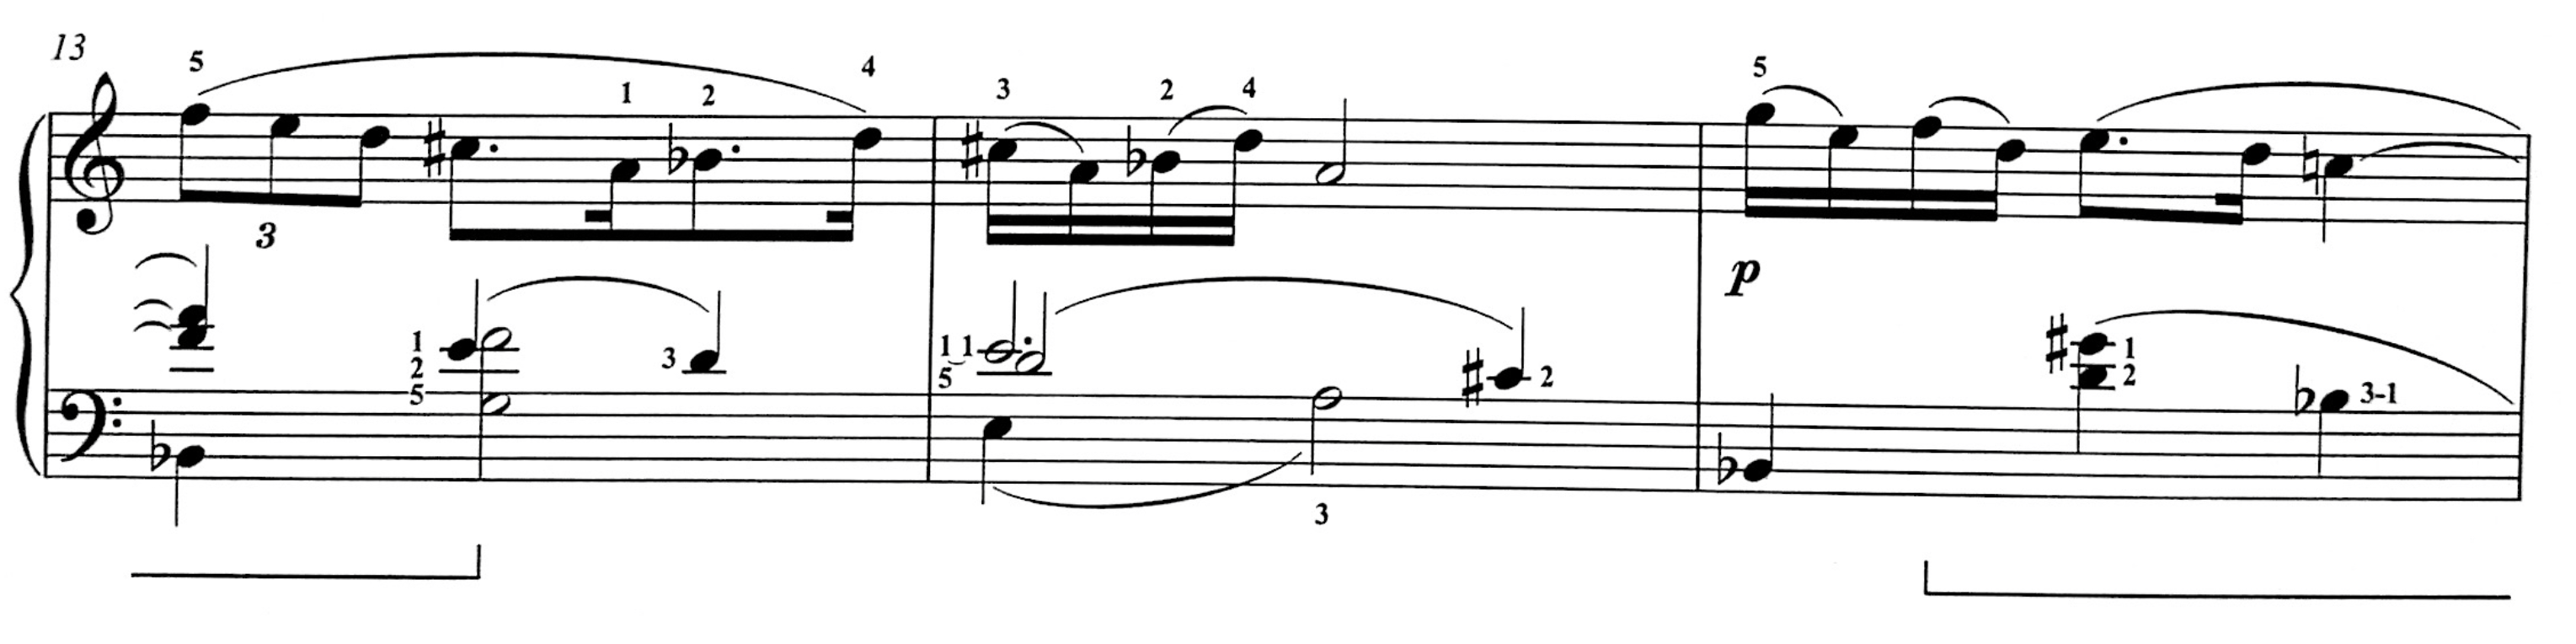
\includegraphics[width=\textwidth]{bartok-dance-four-b-section-second-system.jpg}
  \caption[The second system of ``Buciumeana'' in Bartok's \textit{Romanian Folk Dances, Sz. 56, BB 88}]{The second system of the B section in ``Buciumeana''}
  \label{fig:bartok-dance-four-b-section-second-system}
\end{figure}

The similarities between sections A and B begin after the first two bars of each section. The themes in the sections become visible, as seen in figures \ref{fig:bartok-dance-four-first-line}\autocite{Lung_2016} and \ref{fig:bartok-dance-four-b-section-second-system}\autocite{Lung_2016}. It is only the first two measures of each section which differentiates them. The first two bars of section A begin with a half note and quarter note, followed by an eighth note phrase, while the first two bars of section B begin with a phrase of sixteenth and eighth notes. After these two measures, Bartok uses the same melodic material between the two sections. 

\subsection{``Poarga Românească'' (Romanian Polka)}

\begin{figure}
  \centering
  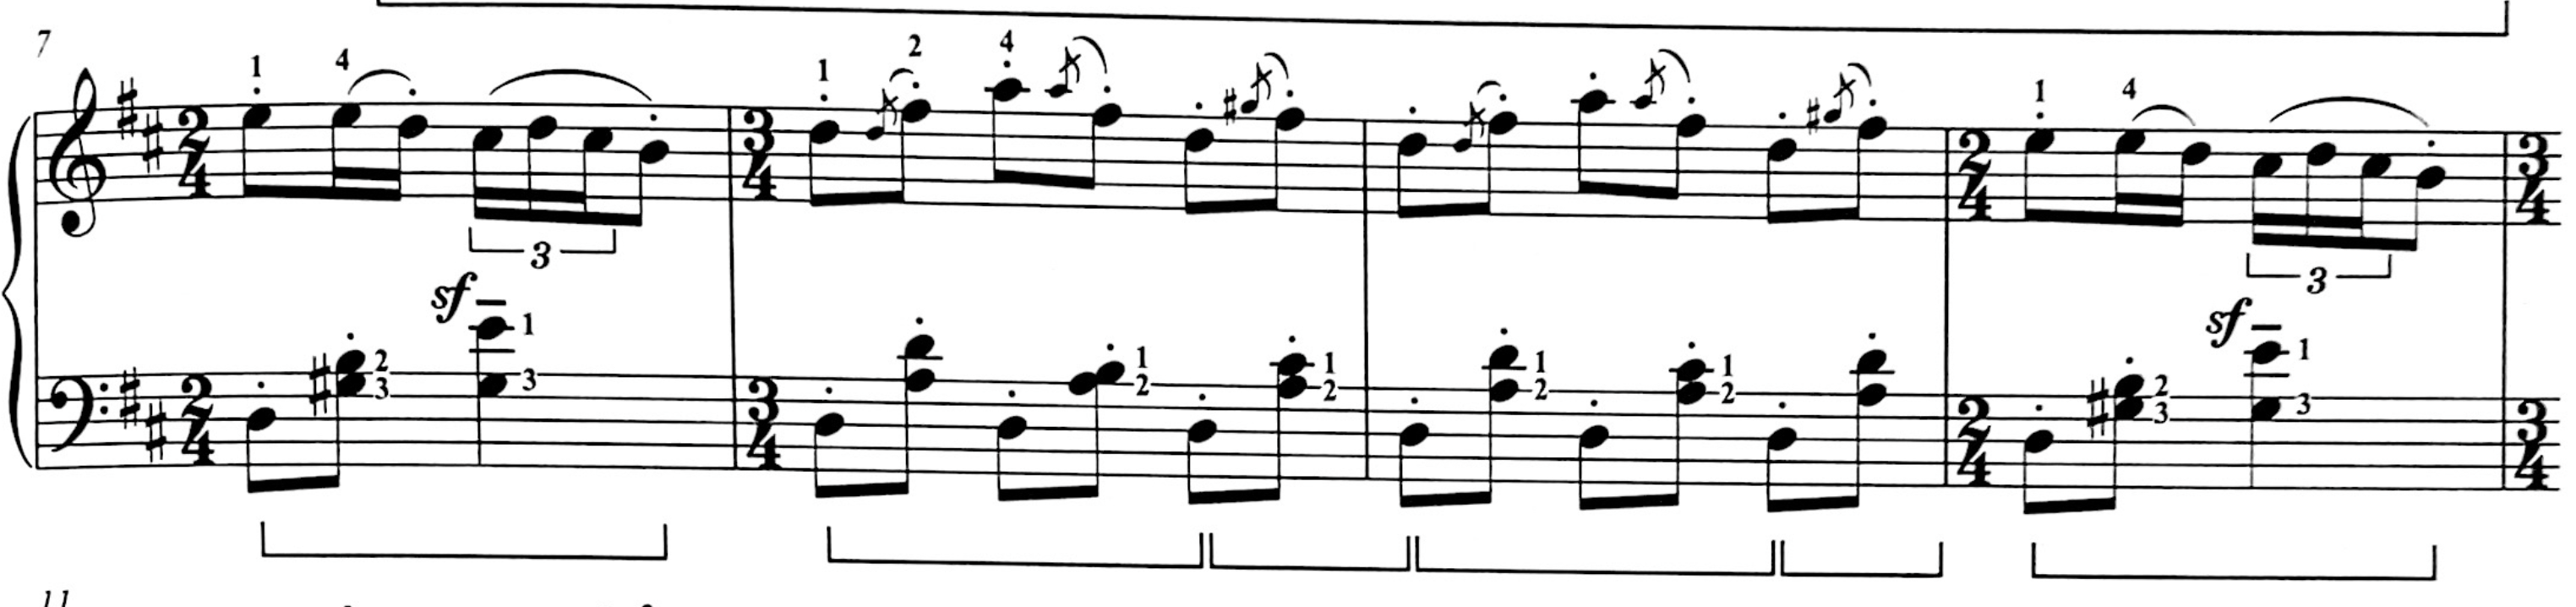
\includegraphics[width=\textwidth]{bartok-dance-five-time-signature.jpg}
  \caption[The alternating meters in ``Poarga Românească'' of Bartok's \textit{Romanian Folk Dances, Sz. 56, BB 68}]{Alternating meters in ``Poarga Românească''}
  \label{fig:bartok-dance-five-time-signature}
\end{figure}

\begin{figure}
  \centering
  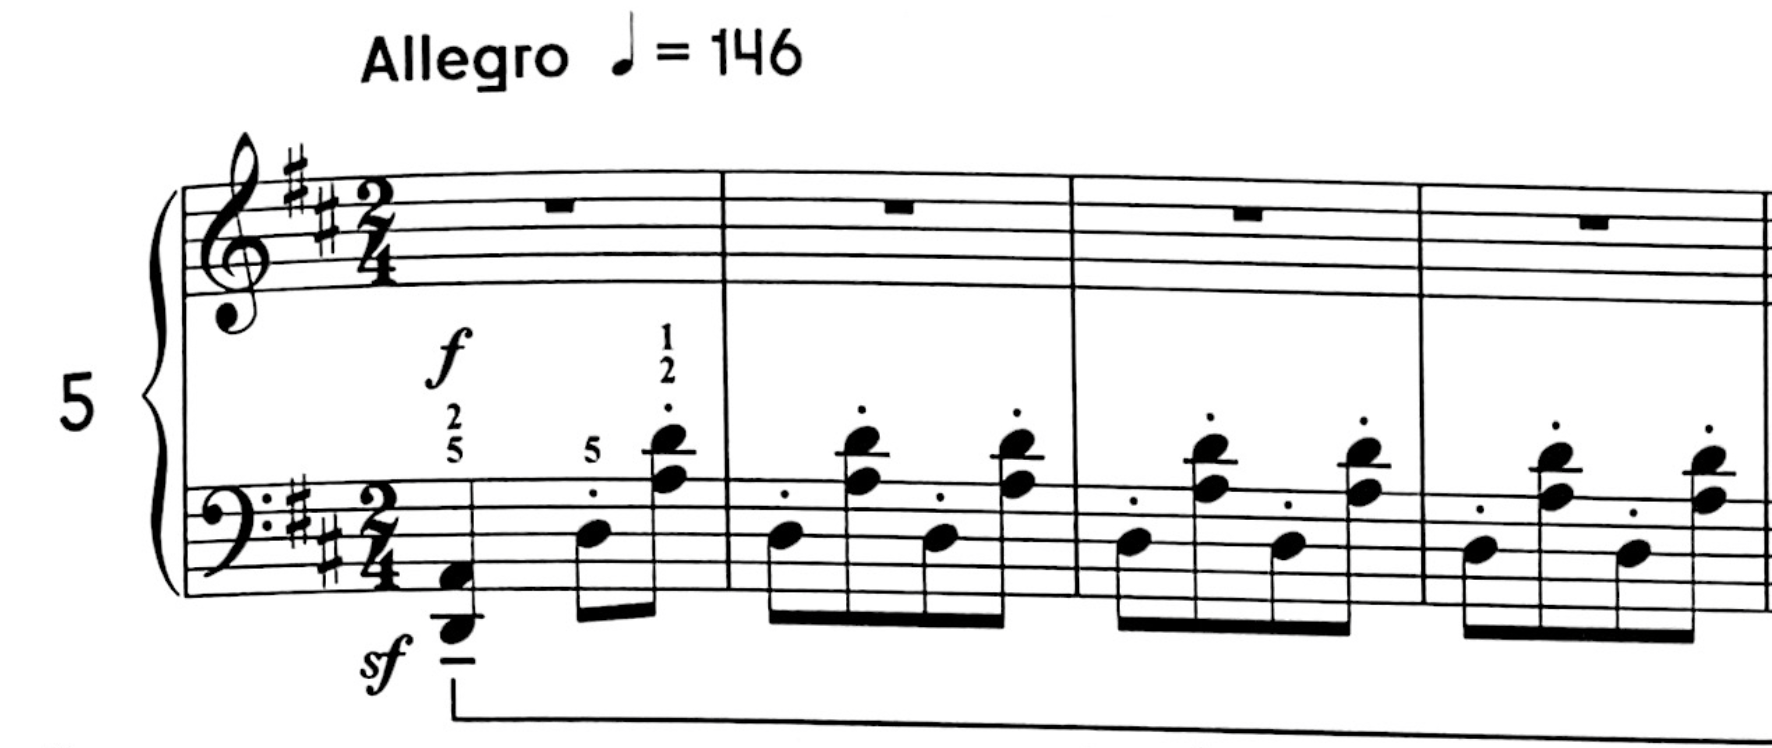
\includegraphics[width=\textwidth]{bartok-dance-five-first-four-bars.jpg}
  \caption[The first five bars of ``Poarga Românească'', of Bartok's \textit{Romanian Folk Dances, Sz. 56, BB 68}]{The first five bars of ``Poarga Românească''}
  \label{fig:bartok-dance-five-first-four-bars}
\end{figure}


The fifth dance, ``Poarga Românească'', comes from modern day Beius, on the border between Hungary and Romania. It is reminiscent of an old Romanian dance similar to the Polka. It is notable as being the only dance in this set with a consistent alternating meter, between $\frac{3}{4}$ and $\frac{2}{4}$, in a pattern of two measures in $\frac{3}{4}$, followed by one measure in $\frac{2}{4}$, as in Figure \ref{fig:bartok-dance-five-time-signature}\autocite{Lung_2016}. This hypermeter (defined as groups of measures which form patterns of accentuation, especially at faster tempos\autocite{Hughes_Gotham_Hamm_2021}) creates a sense of asymmetry, which results in an energetic, continuous-movement in the dance, and a three-measure phrase. The last bar of this three-bar phrase is much shorter than the first two. The piece overall contains an energetic peasant-like dance theme, played in total for about a half-minute in length. The dance starts in the key of D Major, in Figure \ref{fig:bartok-dance-five-first-four-bars}\autocite{Lung_2016}, with the raised fourth scale degree G\musSharp{} (Figure \ref{fig:bartok-dance-five-time-signature}\autocite{Lung_2016}).

\begin{figure}
  \centering
  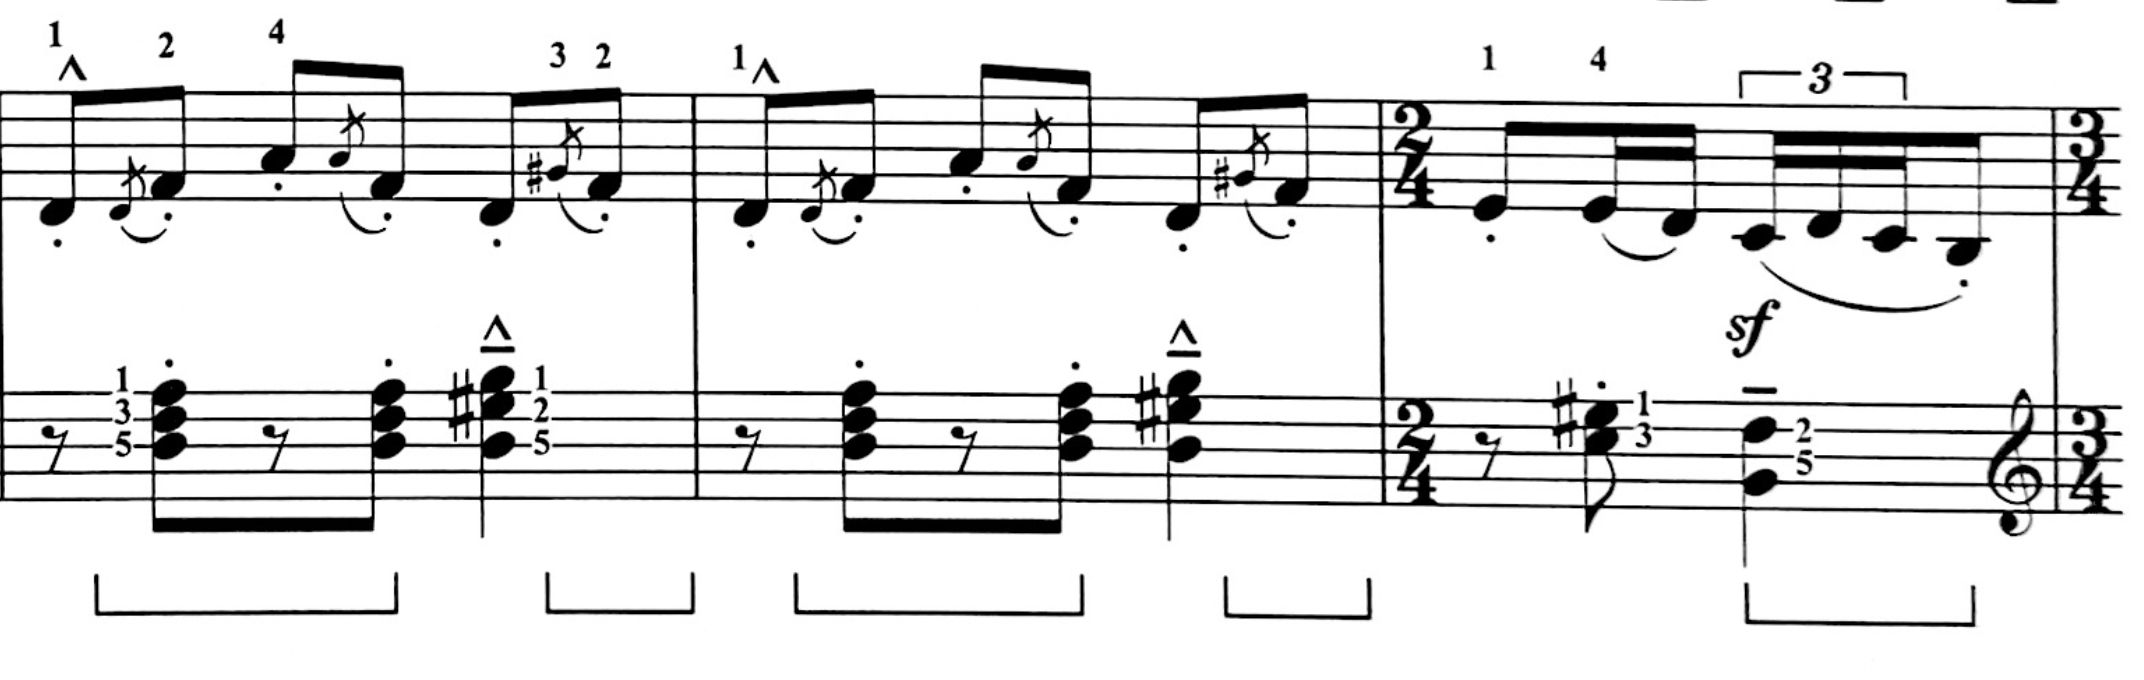
\includegraphics[width=\textwidth]{bartok-dance-five-b-section.jpg}
  \caption[The first three bars in the B section of ``Poarga Românească'' in Bartok's \textit{Romanian Folk Dances, Sz. 56, BB 68}]{The first three bars of the B section in ``Poarga Românească''}
  \label{fig:bartok-dance-five-b-section}
\end{figure}

\begin{figure}
  \centering
  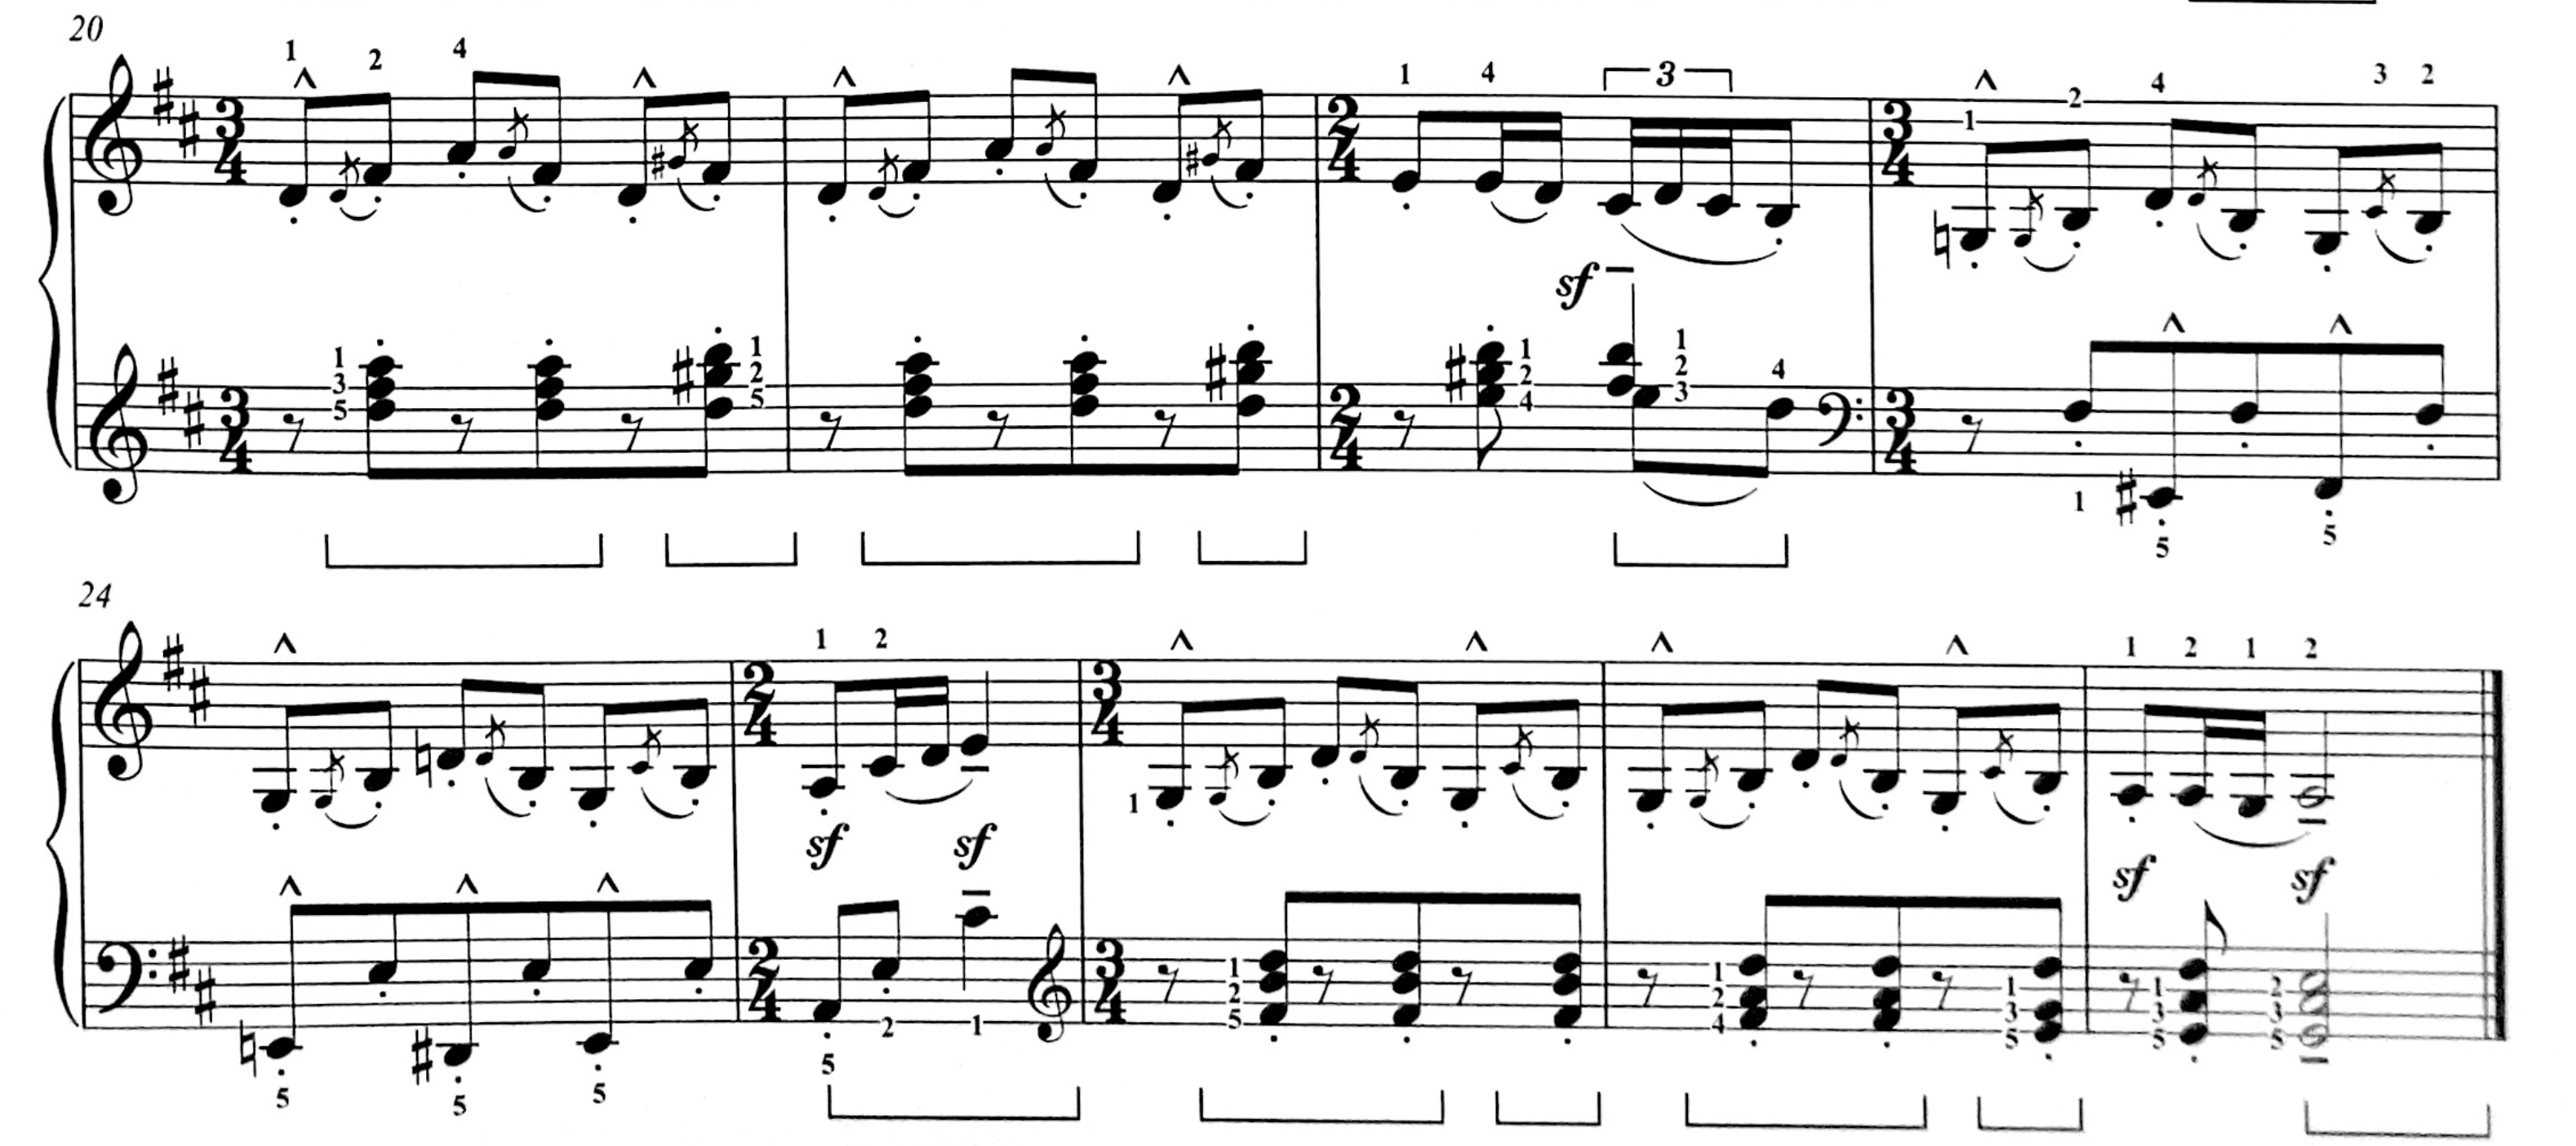
\includegraphics[width=\textwidth]{bartok-dance-five-ending.jpg}
  \caption[The last two systems in ``Poarga Românească'' of Bartok's \textit{Romanian Folk Dances, Sz. 56, BB 68}]{The last two systems in ``Poarga Românească''}
  \label{fig:bartok-dance-five-ending}
\end{figure}


Structurally, this dance is in binary form. Section A lasts from measures 1-16, and section B from measures 17-28. In the A section, the usage of \textit{staccato} and grace notes are two articulation phrases which contribute to the update, danceable nature of the piece. The \textit{staccato}, and thus the sudden bounciness of the note, adds a sense of quickness and dancing energy. The grace notes, as in Figure \ref{fig:bartok-dance-five-time-signature}\autocite{Lung_2016}, also contribute to the high-energy of the piece, with \textit{staccato} notes and slurred notes. In the B section, Bartok introduces syncopation in the left hand's accompaniment, as in Figure \ref{fig:bartok-dance-five-b-section}\autocite{Lung_2016}. A \textit{szforzando} is added to the end of each phrase as a clear ending, such as in the last bar in Figure \ref{fig:bartok-dance-five-b-section}\autocite{Lung_2016}. Then, from bar 20 through to the end of the dance, Bartok writes a \textit{szforzando} every third measure, and in bars 25 and 28, includes a szforzando in the first and third beats of the measure (Figure \ref{fig:bartok-dance-five-b-section}\autocite{Lung_2016}), creating a contrast with the beginning of the piece. 

\subsection{``Mărunțel`` (Fast Dance)}

\begin{figure}
  \centering
  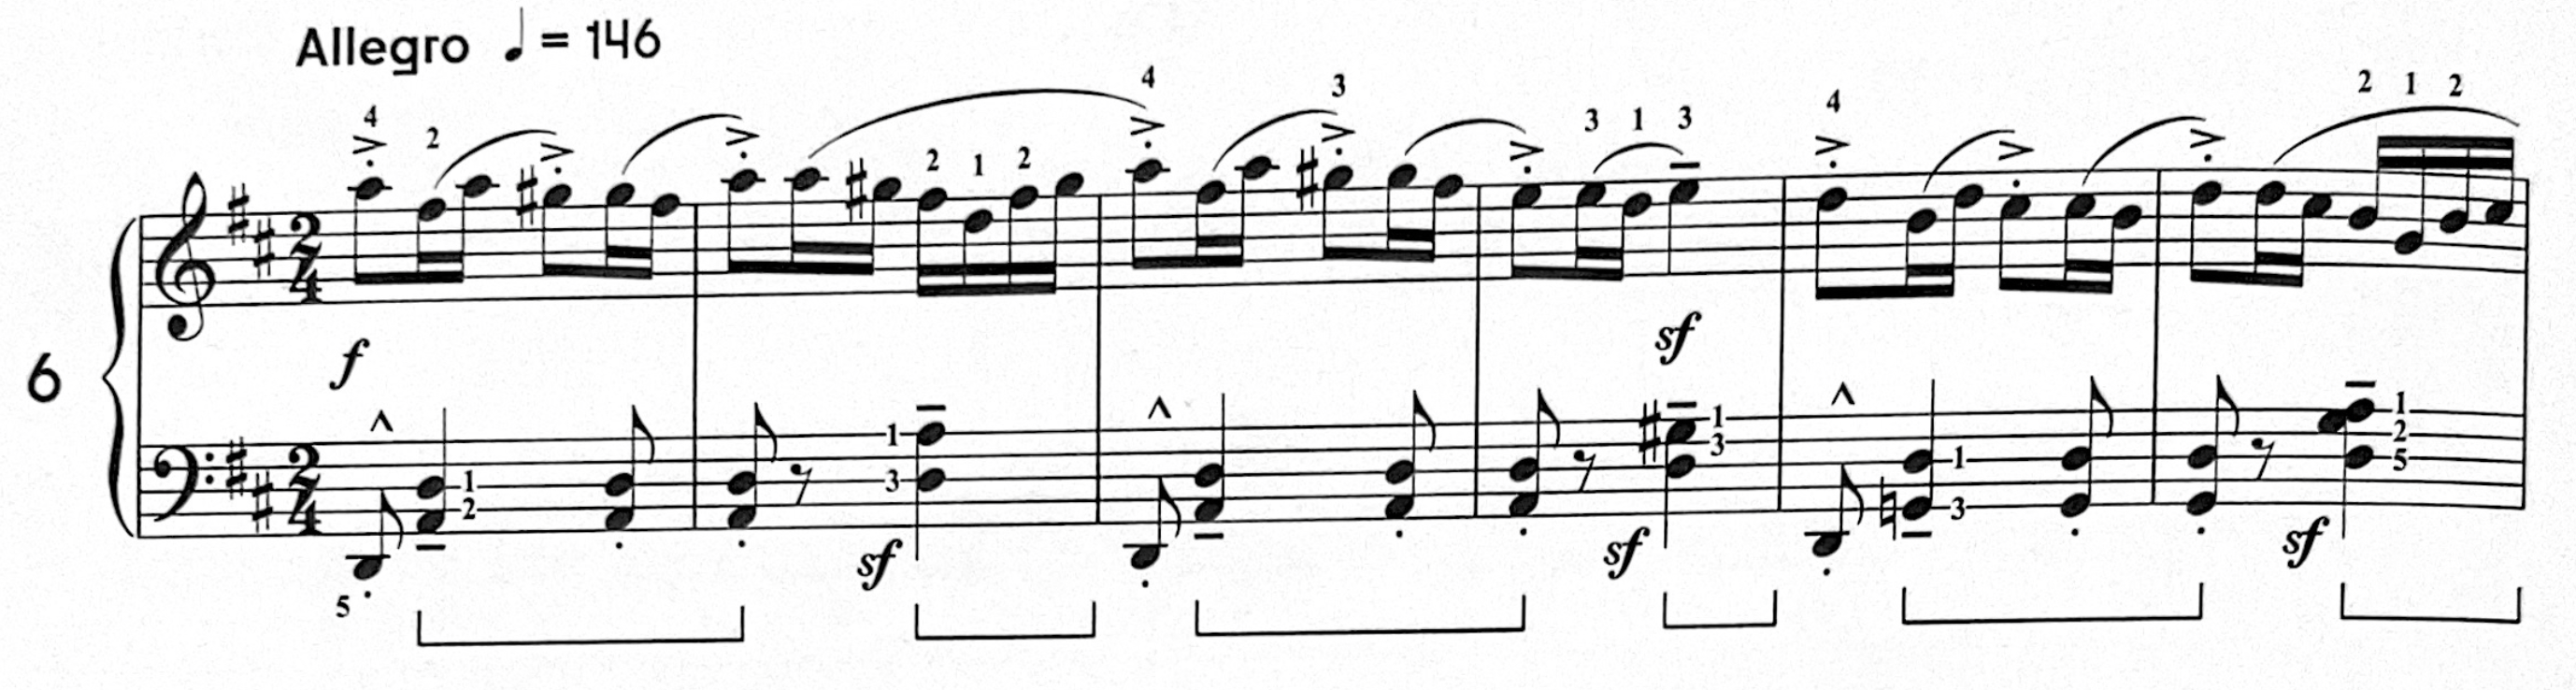
\includegraphics[width=\textwidth]{bartok-dance-six-first-line.jpg}
  \caption[The first line of ``Mărunțel`` of Bartok's \text{Romanian Folk Dances, Sz. 56, BB 68}]{The first line of ``Mărunțel``}
  \label{fig:bartok-dance-six-first-line}
\end{figure}

\begin{figure}
  \centering
  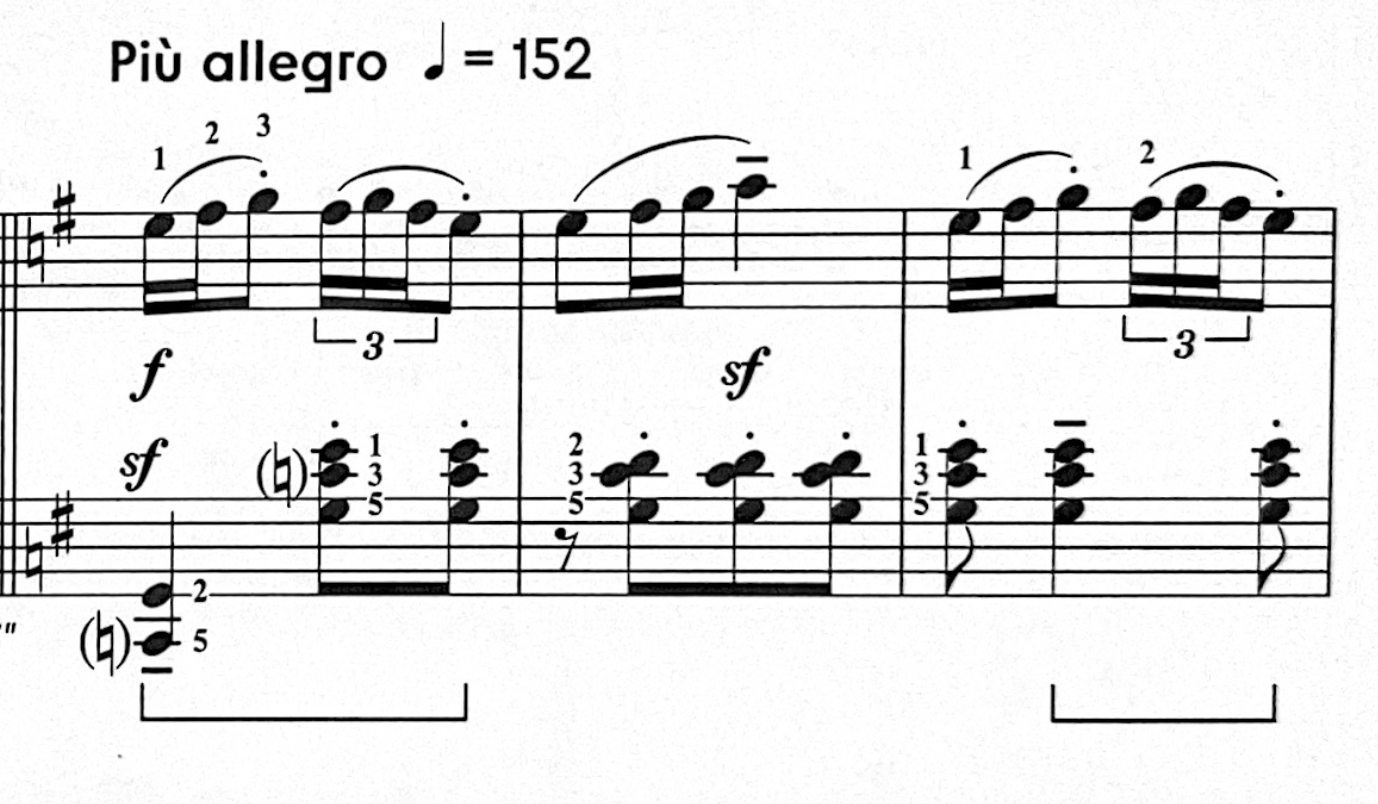
\includegraphics[width=\textwidth]{bartok-dance-six-b-section.jpg}
  \caption[The beginning of the B section in ``Mărunțel`` of Bartok's \textit{Romanian Folk Dances, Sz. 56, BB 68}]{The beginning of the B section in ``Mărunțel``}
  \label{fig:bartok-dance-six-b-section}
\end{figure}

\begin{figure}
  \centering
  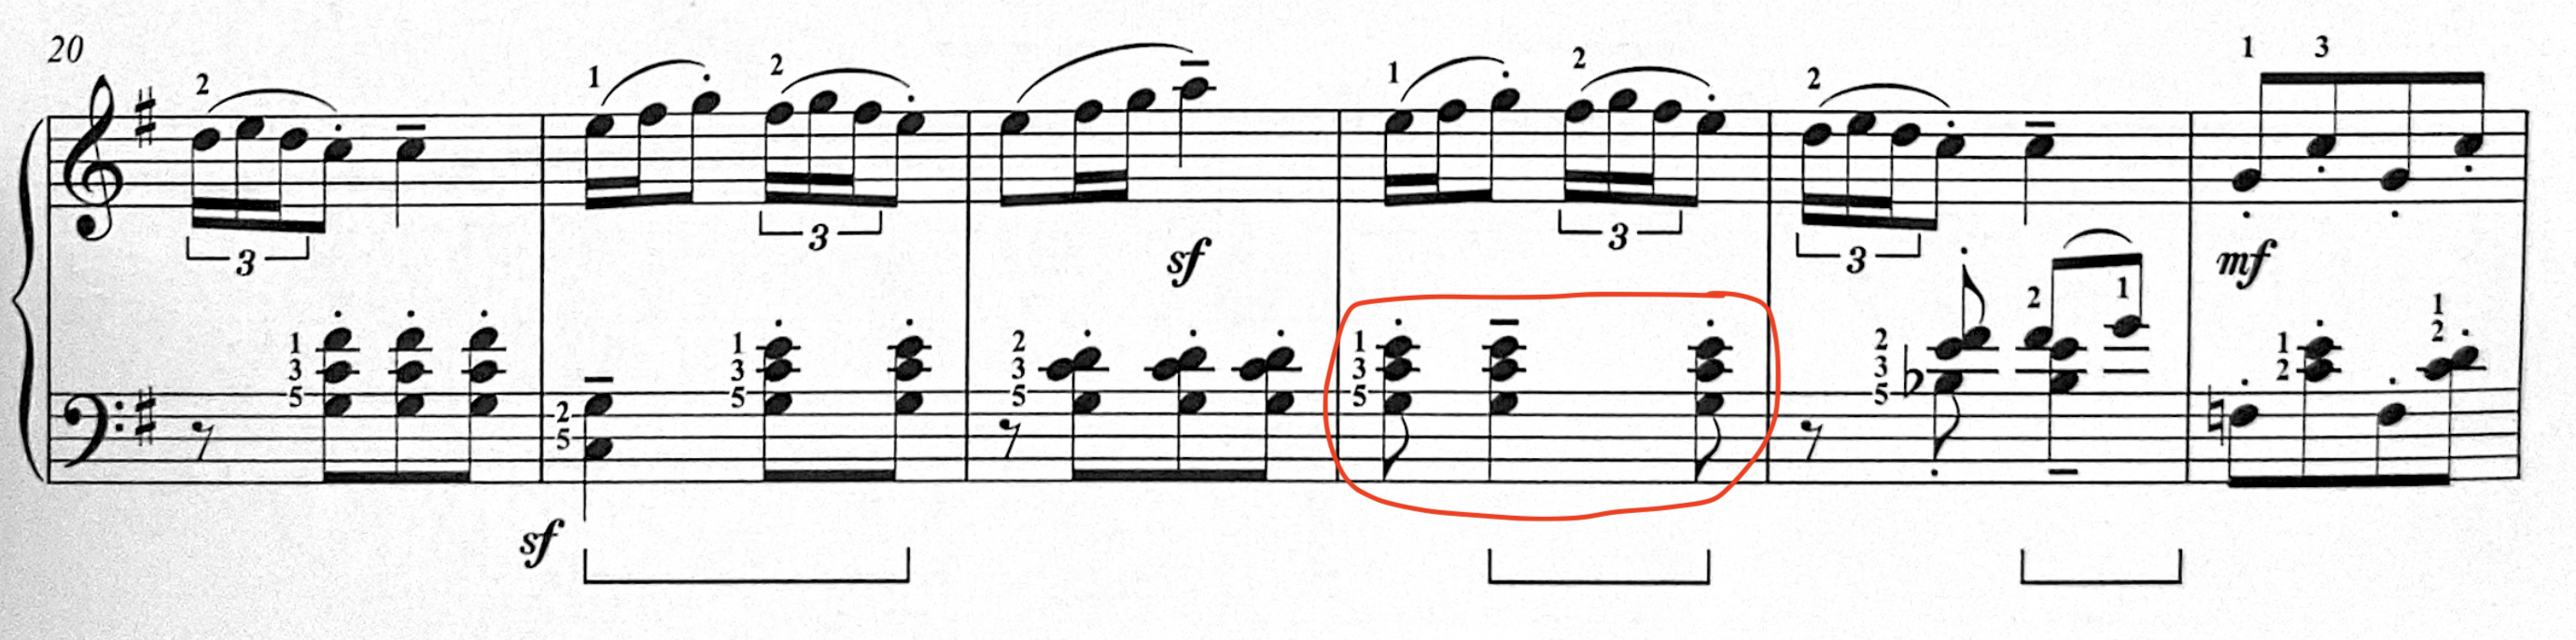
\includegraphics[width=\textwidth]{bartok-dance-six-b-section-syncopation.jpg}
  \caption[Syncopation in the B section in ``Mărunțel`` of Bartok's \textit{Romanian Folk Dances, Sz. 56, BB 68}]{Syncopation in the B section in ``Mărunțel``}
  \label{fig:bartok-dance-six-b-section-syncopation}
\end{figure}


The last dance of the set of six Romanian Folk Dances is ``Mărunțel``, which features two distinct yet similar themes. Each of these themes feels breathless in pacing, as a celebration of some kind without urgency. The beginning of the dance features a narrow melody, each of phrase of which is contained within an octave and uses small steps (Figure \ref{fig:bartok-dance-six-first-line}\autocite{Lung_2016}). As a whole, the piece is written in binary form, with section A lasting from measures 1-16, and section B from measures 17 to the end. The tonic of the piece begins in D Major, and uses a raised fourth scale degree\footnote{We should now be able to recognize the raised fourth scale degree as a feature typical of Romanian folk dances.} G\musSharp{}. At the beginning of the A section, we notice that the melodic line embodies the title of the piece (which in English translates to ``Fast Dance''), which fast melodic and harmonic phrases, as in Figure \ref{fig:bartok-dance-six-first-line}\autocite{Lung_2016}. The fast sixteenth note phrases of the section represent the fast steps dancers would need to perform to keep to the beat of the dance, but must also not be overplayed by the instrumentalist. There are also accents on also every beat to emphasize the $\frac{2}{4}$ time signature of this dance, and to provide balance against the rhythm of the harmony. When the B section begins, there is a change to the tempo, from \textit{Allegro} to the \textit{Più allegro}. There is also an introduction of triplets, which contributes to the higher-energy feeling of the B section. When the dance is played at tempo, these triplets sound as ornamentation, due to the speed at which they are played, as circled in blue in Figure \ref{fig:bartok-dance-six-b-section}\autocite{Lung_2016}. 

The B section is twice as long as the A section, with the melodic material which begins the B section returning in measure 33. However, the material does not return as an exact duplication of the first treatment of the material. There are variations to the left-hand harmony's chord progression, and Bartok eliminates the syncopated rhythm in favor of using the smoother-sounding quarter and eighth notes. By simplifying the accompaniment, the listener can focus on the melody.
